\section{Exercise 4}
Cho mạch điện sau, tính các đại lượng \(I_1\), \(I_2\), \(I_3\), \(V_a\), và \(V_b\).
Trình bày các bước tính toán và kiểm tra bằng mô phỏng.
\begin{figure}[!htbp]
    \centering
    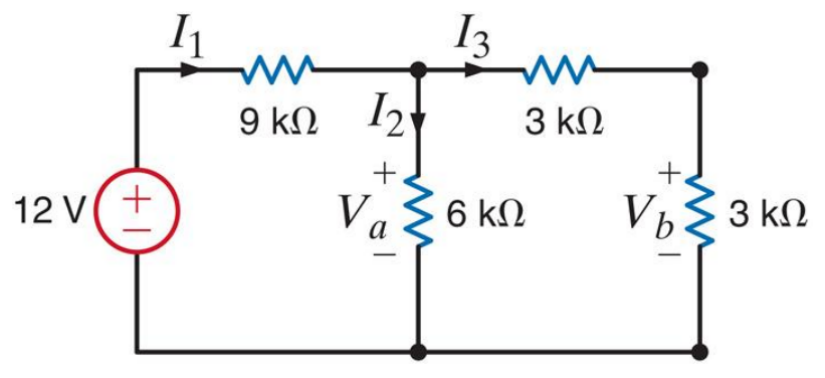
\includegraphics[width=0.7\textwidth]{graphics/ex4/f1.png}
    % \caption{Mạch ban đầu}
\end{figure}
\subsection{Tính toán}
\textbf{Ghi chú}:

Cung cấp giải thích, công thức và phương trình dẫn đến kết quả.

\textbf{Lời giải}

\begin{itemize}
    \item Điện trở tương đương (equivalent resistance) của cả mạch:
    \[
    R_{eq} = \frac{(3k\Omega + 3k\Omega) \cdot 6k\Omega}{(3k\Omega + 3k\Omega) + 6k\Omega} + 9k\Omega = 12k\Omega.
    \]
    \item Dòng điện \(I_1\) được tính như sau: \(I_1 = \frac{V}{R_{eq}} = \frac{12V}{12k\Omega} = 1 mA.\)
    \item Áp dụng định luật Kirchoff cho điện áp (KVL) trong vòng kín trên hình: 
    \begin{figure}[!htbp]
        \centering
        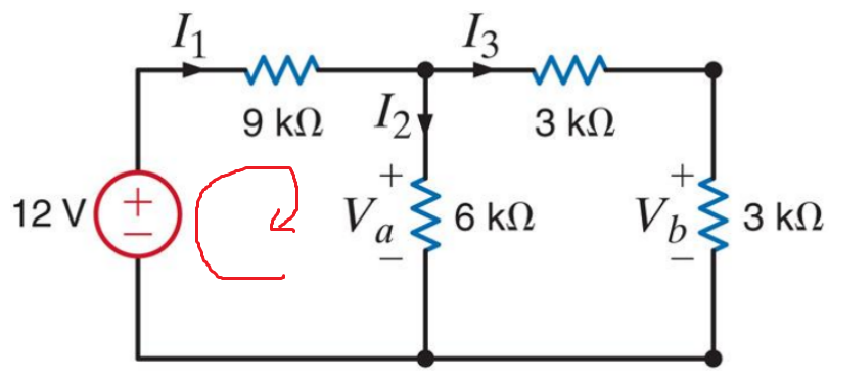
\includegraphics[width=0.7\textwidth]{graphics/ex4/f1a.png}
    \end{figure}
    \[
    I_1 \cdot 9k\Omega + I_2 \cdot 6k\Omega = 12V
    \longrightarrow I_2 = \frac{12V -  I_1 \cdot 9k\Omega }{6k\Omega} = \frac{12V -  1mA \cdot 9k\Omega }{6k\Omega} = 0.5 mA.
    \]
    \newpage
    \item Áp dụng định luật Kirchhoff cho dòng điện (KCL) cho nút trên hình:
    \begin{figure}[!htbp]
        \centering
        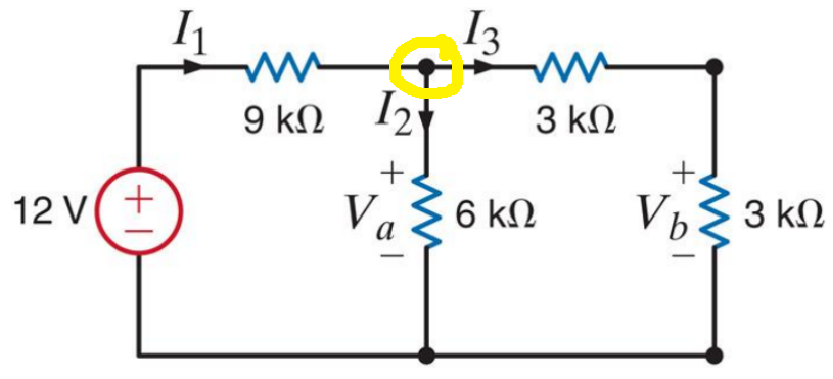
\includegraphics[width=0.7\textwidth]{graphics/ex4/f1b.png}
    \end{figure}
    \[
    \displaystyle \sum i_{in} = \sum i_{out}
    \longleftrightarrow I_1 = I_2 + I_3
    \longrightarrow I_3 = I_1 - I_2 = 1mA - 0.5mA = 0.5mA
    \]
    \item Vì \(I_2\) và \(I_3\) có giá trị dương, nên chiều các dòng điện đúng như ký hiệu trong mạch. Do đó, 
    \(V_a = -I_2 \cdot 6k\Omega = - 0.5mA \cdot 6k\Omega = -3V\)

    \(V_b = -I_3 \cdot 3k\Omega = - 0.5mA \cdot 3k\Omega = -1.5V\) 
\end{itemize}

\subsection{Mô phỏng}
Kết quả mô phỏng:
\begin{figure}[!htbp]
    \centering
    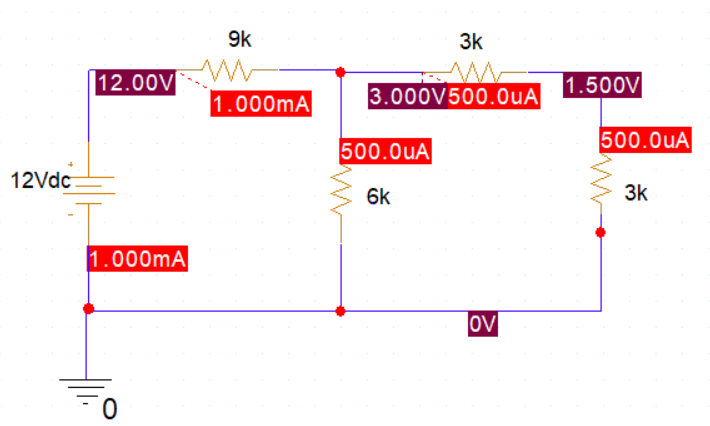
\includegraphics[width=0.7\textwidth]{graphics/ex4/f2.png}
\end{figure}

